% NSF proposal generation template style file.
% based on latex stylefiles written by Stefan Llewellyn Smith and
% Sarah Gille, with contributions from other collaborators.
%
\documentclass{proposalnsf}

% See this file for a set of pre-defined journal abbreviations
\newcommand{\jas}{{\it J. Atmos. Sci.}}
\newcommand{\jpo}{{\it J. Phys. Oceanogr.}}
\newcommand{\JPO}{{\it J. Phys. Oceanogr.}}
\newcommand{\jfm}{{\it J. Fluid Mech.}}
\newcommand{\jgr}{{\it J. Geophys. Res.}}
\newcommand{\JGR}{{\it J. Geophys. Res.}}
\newcommand{\jmr}{{\it J. Mar. Res.}}
\newcommand{\arfm}{{\it Ann. Rev. Fluid Mech.}}
\newcommand{\dsr}{{\it Deep-Sea Res.}}
\newcommand{\dao}{{\it Dyn. Atmos. Oceans}}
\newcommand{\jam}{{\it Journal of Applied Meteorology}}
\newcommand{\phfl}{{\it Phys. Fluids}}
\newcommand{\phfla}{{\it Phys. Fluids A}}
\newcommand{\PhilTrans}{{\it Philosophical Transactions of the Royal Society, London}}
\newcommand{\gafd}{{\it Geophys. Astrophys. Fluid Dyn.}}
\newcommand{\gfd}{{\it Geophys. Fluid Dyn.}}
\newcommand{\PCE}{{\it Physics and Chemistry of the Earth}}
\newcommand{\PRL}{{\it Physical Review Letters}}
\newcommand{\ProgOc}{{\it Prog. Oceanography}}
\newcommand{\WHOITR}{Woods Hole Oceanographic Institution Technical Report, WHOI-} 
\usepackage{hyperref}
\usepackage{xcolor}
\usepackage{graphicx} 
\newcommand{\keyword}[2]

\newcommand{\degrees}{$\!\!$\char23$\!$}
\newcommand{\armin}[1]{\colorbox{cyan}{#1}}
\newcommand{\austin}[1]{\colorbox{yellow}{#1}}
\newcommand{\greg}[1]{\colorbox{orange}{#1}}
\newcommand{\josh}[1]{\colorbox{green}{#1}}
\newcommand{\red}[1]{\colorbox{red}{#1}}
\newcommand{\ana}[1]{\colorbox{red}{#1}}
\newcommand{\changeit}[1]{\colorbox{magenta}{#1}}

\newcommand{\eg}{\emph{e.g.}}
\newcommand{\id}{\emph{i.d.}}

\renewcommand{\refname}{\centerline{References cited}}

% This handles hanging indents for publications
\def\rrr#1\\{\par
\medskip\hbox{\vbox{\parindent=2em\hsize=6.12in
\hangindent=4em\hangafter=1#1}}}

\def\baselinestretch{1}

\begin{document}
{\LARGE{
\noindent
\armin{Armin please review}\\
\austin{Austin please review}\\
\greg{Greg please review}\\
\josh{Josh please review}\\
\ana{Ana please review}\\
\changeit{To be changed}}}

\clearpage
\begin{center}
{\Large{\bf Project Summary}}\\*[3mm]
{\bf AI detecting echoes of stellar explosions in the LSST data} \\*[3mm]

Federica B.  Bianco, PI; 
Austin J.  Brockmeier, 
Armin Rest, CoIs; \\
Gregory Dobler, 
Joshua Peek, Collaborators
\end{center}
\vspace{-3mm}
{\bf Overview} This is a proposal to build a pipeline for blind all-sky scale automated detection of light echo to be deployed on the LSST computational platform. The detection of light echoes at scale will enable studies of the Galactic dust and of the history of stellar explosions and eruptions in the Galaxy.

\noindent
{\bf Intellectual Merit} The Large Synoptic Survey Telescope (LSST) is the US flagship astronomical project of the 2020s.   LSST will conduct a 10-year survey generating an unprecedented amount of information-dense data: 20Tb/night, every night, for 10 years, pushing the envelope of big-data and data-science.   Covering the whole southern sky every few days, the LSST data reduction software will detect tens of thousands of transients in the sky every night, but it will entirely miss \emph{light echoes}: the reflection of stellar explosions that light up cosmic dust.   The detection of all-sky samples of light echoes (LEs) enables the reconstruction of the history of explosions in our Galaxy, including the potential to detect an unknown galactic supernova, and the tracing of the Milky Way dust structure, which informs the evolution history of the Galaxy and improve inferences on extragalactic sources by constraining extinction.  However, LEs are faint, rare, and diffuse features that change over time, and are hard to detect.  Presently, no automated pipeline for this task exists.  LSST will observe the entire southern sky at $\sim$day time intervals and with high sensitivity and spatial resolution, making it the ideal survey to detect LEs.  This program will support the development of the first pipeline for the automated all-sky detection of LEs by leveraging cutting-edge artificial intelligence, and its deployment on the LSST computing platform.  The products of this work will be primarily: (1) a method to detect LEs in all sky images optimized for LSST and implemented on the LSST platform as a User-Generated data product. (2) A census of LEs on the Galaxies which will be combined with eruption and explosion models to constrain the history of eruption and explosion of the Milky Way. (3) An AI based method to generate detailed, spatially resolved dust maps automatically in correspondence to LEs detected.

\noindent
{\bf Broader Impacts}
This proposal will leverage the fascinating phenomenon of LEs to develop data science skills.  It will provide research and training opportunities for graduate and undergraduate students.  The involvement of CoI Brockmeier (Assistant Professor of Electrical and Computer Engineering), and the connection of PI Bianco, CoI Brockmeier, and Collaborator Dobler with the new UD Data Science Institute will provide an immersive environment where our students can benefit from mentoring opportunities, as well as opportunities to share their work on a regular basis (\eg annual Data Science Symposia).   Furthermore, the CoIs will develop a hackathon program for University of Delaware students that will provide prime active learning experiences, a unique venue to get exposed in data science, and opportunities to prototype solutions for LSST data analysis. But not limited to LSST or even astrophysics, offering data science projects across disciplines.  This learning environment is ideal to develop superskills not generally offered in the classroom or in traditional research projects: from project scoping and design, to collaborative and communication skills.
\renewcommand{\thepage} {B--\arabic{page}}

%\newpage

% reset page numbering to 1.   This is helpful, since the text can only
% be 15 pages, and reviewers will want to believe we've kept within
% those limits

\pagenumbering{arabic}
\renewcommand{\thepage} {D--\arabic{page}}

\newpage

\centerline{\bf Results from Prior NSF Support}

\noindent
{\bf Previous Award Title}
{\it award number} (PI); dates, \$amount

Research carried out ....


\noindent{\Large \bf PROJECT DESCRIPTION}

\section{Introduction}


About a century ago a true paradigm shift happened in astronomy.   The introduction of digital equipment enabled the discovery and study of the “transients and variable sky” : the sky that in all human mythologies was assumed to be never-changing came to life with the detection of energetic phenomena happening every instant: 10 stars explode every second [a], stars merge deforming space-time in gravitational waves [a], they erupt [a], and more.   A century ago seeing an astronomical transient was a once-in-a-lifetime event, now we see many-a-day, and yet we have barely scratched the surface of this scientific opportunity.  Until now, astronomical surveys were limited in either depth, only enabling the observation of the closest and brightest transients, area, observing small regions of sky, or resolution.   Today we can detect ~100 transients each night [4].   LSST will detect tens of thousands, representing not an incremental, but a transformational change.  

{\bf The LSST project} includes the construction of a telescope and a 10-year survey to begin in 2022 [5].  LSST will deliver an unprecedented volume of information-dense data (20Tb/night) with the potential to revolutionize nearly all astrophysics domains [6], from revealing the smallest bodies in the Solar System, to measuring the rate of expansion of the Universe.   LSST will photograph the sky at resolution and depth comparable to those of the Hubble Space Telescope, but unlike previous surveys, limited to small regions, it will deliver observations at a few days’ cadence over the whole southern sky.   This will truly open a window into the transient Universe.  

{\bf Light Echoes} (LEs) are the reflection of stellar explosions on interstellar dust.  They appear in the sky as diffuse transients: faint, extended, time-varying [7].  
As part of its federally funded operations, LSST will produce $10^6$ nightly alerts, each one announcing a changing or moving source (stars, asteroids, etc).   It will detect thousands of transients and variable “point sources” in each image but these diffuse features will be entirely missed.   LEs help characterize stellar explosions by offering the view of an explosion from different lines of sight, a unique opportunity in astrophysics [8,9] 
 and allowing us to revisit events even when the transient was originally not detected [10].  
{\bf\emph{ The detection of LEs across a large portion of the sky enables the reconstruction of the history of stellar explosions of our Galaxy, the potential to detect an unknown galactic supernova, and the tracing of the Milky Way dust structure, which will inform the evolutionary history of the Galaxy and improve inference on extragalactic sources by constraining extinction.  }}


{\bf However, LEs are extremely hard to detect}, and, to date, they are still discovered by visual inspection, a method that obviously does not scale to the LSST data volume.   Even crowd-sourcing cannot help this science in the LSST era: simple scaling from the Galaxy Zoo \ana{[CITE]} project indicates that the entire population of the Earth would be insufficient to study the full dataset using the same methods.   We propose to leverage Artificial Intelligence to address this low signal-to-noise regime computer-vision challenge and create the first pipeline for automated detection of LEs.   {\bf \emph{This will allow us to use images from the LSST survey to produce a census of LEs that would constrain the history of Milky Way stellar explosions, and create detailed map dusts everywhere light echoes are found}}.

This proposal will support the development of an Artificial Intelligence (AI) model, a Generative Adversarial Neural Network [15], to detect LEs at scale in the LSST data.   Deep Neural Networks and AI have recently been employed to solve astronomical tasks, primarily due to the rapid increase in data volume, which will culminate with the LSST survey and which requires scalable models that can efficiently extract information from Terabytes of data [\eg,  16].   Over the course of the next two years we expect to develop a model to detect LEs automatically in sky images and test the model on LSST precursor surveys.   Attempts to develop software to automatically detect LEs that are based on human-engineered features in images have not been successful, and by far the best method to detect LEs to date is human-inspection.  However, human-inspection obviously cannot scale to the volume of data generated by LSST and to the scope of the problem we ultimate propose to approach: the creation of a comprehensive census of Galactic LEs to study the history of stellar explosions and eruptions in the Milky Way.   

This work will constitute a core portion of the PhD Thesis of one of PI Bianco’s graduate students at the DPA.   We will start from the limited size sample of real light-echo examples, a dataset of simulated LEs generated analytically, and images of the underlying dust wherever available (infrared observations of the sky reveal dust features, but high-resolution images are not available across the entire sky).   We will use successful Generative Adversarial Neural Networks designed to work under similar circumstances of limited-size real examples and simulated data [18].   Our team will retrain this network on light echo images from telescopes systems similar to the LSST (\eg,  from the Blanco telescope Dark Energy Camera, DES, images obtained in proposals co-authored by PI Bianco), and change the network architecture to suit our needs.  We expect to be able to test our model on real data as soon as commissioning data from LSST will become available.   In the meantime, our software can run on existing Blanco/DES images, that share many of the crucial characteristics of the LSST data but are not as sensitive to faint magnitudes, leading to a lower detection rate, looking for known and unknown LEs.


The two-year timeline of this proposal aligns perfectly with LSST, whose first commissioning data are expected in 2021 and which will begin observing in 2022.   The work to be conducted under this proposal will produce important software that will allow us to ``hit the ground running'' and begin detecting LEs in LSST images as soon as the LSST survey begins to produce data.  


\section{\armin{ Light Echoes phenomenology and significance}}
LEs are the reflections light from astrophysical transients off interstellar dust in their surroundings.   As the light from a transient propagates into space, it may be reflected towards Earth, and our telescopes, if it encounters a sheet of interstellar dust.  The geometry of LEs is straightforward, a transient and the Earth are at two focal points of a 3D ellipsoid; light from the transient reflected off dust that intersects the same ellipsoid surface reaches Earth at the same time.  As time goes by, the ellipsoidal surface expands.  Due to the extra travel time, a light echo reaches the observer at a later time than the light directly detected from its source.

LEs appear as faint, extended, time-changing features in the sky.  The complexity of their shape is inferred by the complexity of the underlying dust structure, while the time-changing aspect is due to the traveling of light across the dust sheet.

LEs provide unique insight into the transients that originated them and the dust that produced them.  
\subsection {Nature of the transient}
The nature of transients can be studied in detail in their LEs: this technique has enabled the characterization of historical supernovae with modern instrumentation [8,19,20].  When historical transients are observed (again) today in LEs, they can be studies with modern observing techniques: large telescopes, with aperture that compensate for the factor $10$ decrease in brightness, digital cameras, and, most importantly, spectrographs that enable typing and the characterization of physical properties of the transient that cannot be inferred from overall magnitude measurements.  For examples: the historic Tycho supernova, was first observed in northern Europe in 1572.  At the time, the concept of stars having a finite life-time was many years to come.  When re-detected in 20??, a study lead by CoI Rest identified the explosion as a supernova of type Ia (SNIa), through the analysis of the spectral features of the LE.  These studies 
require a sophisticated modeling of the dust reflection effects to deconvolve the imprint of the dust from the spectrum of the transient (or rather, to convolve the spectra of directly observed transients with a kernel reproducing the effects of dust and enable comparisons).  CoI Rest is the foremost world expert in this technique \citep{rest11a}.

A blooming field of LEs, detected by our team in the surrounding of Eta Carinae, simply revolutionized our understanding of the nature of this transient, generating numerous publications and radically new models to explain the stellar eruption \changeit{[cite all Eracar including Owocki]}

\subsection{Asymmetry}
LEs, specifically the reflection of astronomical transients onto interstellar dust, enable the study of a transients from multiple lines of sight, a unique opportunity in astrophysics, allowing insight into the physical mechanism of stellar eruptions and explosions [3,8,9,19,20].  Cassiopea A (CasA) stands as a prime example of this: as for other supernova remnants, the remnant of CasA shows signs of asymmetry \changeit{[CITE]}.  But asymmetries in a remnant may be imprinted during the expansion of the ejecta.  CasA LEs, however, which are available from different lines of sight, have provided evidence that the explosion itself was asymmetric, a crucial piece of information to constrain explosion models.  Our team not only conducted the original study that detected the asymmetry signatures in spectra of CasA from different LEs \tochange[RESTCASA], but we also conducted subsequent studies that related the diversity in the sample of obswerved supernova IIb \tochange[Finn], the same type as CasA, to the asymmetry of CasA, demonstrating that the amount of asymmetry measured in CasA is itself comparable to the spectral diversity observed over N SNe IIb.

\subsection{Dust}
\armin{Armin can you add to this?}
The study of the dust structure that reflects the light allows us to characterize and study stellar eruptions through the characteristics of the ejection of material [21].

The iconic images of supergiant start V838 Monocerotis are the most astounding example of LEs revealing the dust structure around a variable\footnote{\url{https://en.wikipedia.org/wiki/V838_Monocerotis}}. 

LEs have been facilitated the study of \armin{[words words words]}

Of course, high signal-to-noise ratio LEs such as that one not the target of this proposal. With this proposal we aim at detecting faint light echoes, such that we can construct a and extracting info from a large sample, really the first statistical sample of LEs. 


\changeit{probably remove cause not relevant but cool:} Recently, LEs have been leveraged even to detect planets around low mass stars (\citep{sparks2018})

\subsection{What detection of LEs at scale enables}
All of these lines of inference are afforded by the study of individual LEs, but due to its sensitivity and all-sky observing strategy, LSST will for the first time enable observation of very faint phenomena on all-sky scale.  
On the long term, the detection of LEs on a large scale across the entire sky will enable several science projects.

\begin{itemize}
  \item 
LEs may reveal unobserved Galactic supernovae.  
 \item 
LSST we expect to be able to do something unprecedented: build a census of Galactic LEs that will allow us to reconstruct the history of explosions and eruptions of the Milky Way, providing insight into the evolution of our Galaxy.   
\item Since all Galactic dust shines in reflected light, however faintly, the detection of LEs will also enable the study of the Galaxy dust structure on large scale.   In combination with studies of the structure from stellar extinction (its ability to absorb light [22]) this will provide an unprecedentedly detailed, three-dimensional map of the Galactic dust which will inform studies of Galaxy formation and improve the characterization of any observed extragalactic source.  
\end{itemize}

\section{Automating the detection of light echo in the LSST era}

\subsection{\armin{The specific challenges in the detection light echo}}


The astronomical community has very specific computer vision needs : common preprocessing tasks like rectifying, stitching, and bundling have been perfected for the low signal-to-noise sparse images that are the norm in astronomy.  Similarly, difference imaging and the detection of changes has seen development since the very early computational methods developed in the 1990s~\citep{alardlupton99} and, combined with machine learning tasks for increasing the purity of the detections~(\citealt{wozniak13} and most recently \citealt{duev19}).  With decades of experience in the study of astronomical transient in digital sky images, specialized software has been perfected to enable the discovery of astronomical transients to high sensitivity, even in real time.  This directly leads to the expectation that the LSST alert stream will be capable of delivering a stream of 10 million time-domain events per night, from transiting exoplanets, to gravitational microlensing, to the most distant explosions, every night, delivered within 60 seconds of closing the shutter.  Delivered to the entire world! for follow up and further investigation.  But this stream of alerts will miss LEs entirely.

The vast majority of astronomical transients are “point sources”, and detection software, including the LSST pipelines, are optimized for the detection of these point-source transients.



In addition, LEs are rare, or rather: LEs that are bright enough to be detected by present surveys, that are not as sensitive, or not as broad as LSST, are rare.  
{\bf LSST will usher a new era in the study of LEs by observing the entire hemisphere sky repeatedly at high spatial resolution and high sensitivity (limiting single-image depth magnitude g~24).  }

The detection of LEs is a difficult computer vision problem.   The problem is similar to the well-known, and notoriously difficult problem of detecting smoke-stacks and plumes, which PI Bianco also worked on in the context of Urban Science with a deep learning approach similar to the one proposed here (at the Urban Observatory [17]).  
The challenges include:
\begin{itemize}
  \item these features have diverse and time-changing shapes, depending on the underlying dust structure and on the travel speed of the light across the dust, itself dominated by line-of-sight effects;
  \item reflections inside the telescope constitute a significant source of false positives, which cannot be disambiguated within a single image and requires time sequences to be analyzed.
  \item LEs appear as faint and diffuse features, ranging in luminosity until they blend into the image noise.   This problem is distinctly different from most image detection and recognition tasks, where the presence of the target object is unambiguous, and resolution is the most likely limiting factor.   
  \item the training set is limited: a few hundred examples.   This is a particular challenge in machine learning and artificial intelligence approaches. 
  \end{itemize}
 For these reasons the automation of the detection of LEs continues to lag behind in an increasingly automated astrophysics discovery chain that for most transients now includes the entire process from detection to follow-up management~\citep{street18}. The first attempt to build a model for automated detection of light echoes is being undertaken under NSF grant 1814993, lead by CoI Rest. However, the automation of LE detection \emph{at scale} in the LSST era is a substantially more complex problem: the LSST data will constitute a "blind", all-sky, LE survey that will gather the equivalent of the entire dataset that constitutes the basis of NSF Grant 1814993 in as little as 3 weeks, and continue to observe for 10 more years. The detection of LEs in LSST images requires an efficient, flexible, reliable pipeline that would need to be deployed on the LSST computational platform as a UG data product, complying to the computational requirements of LSST UG data products and able to perform on LSST images without overwhelming the shared resources that LSST will make available to the US community ad part of their federally funded operations. 



\subsection{The LSST data and user generated data products}


The LSST 10-year survey, to start observing in 2022, is the US flagship ground-based astronomical project of the 2020s: the 2010 report “New Worlds, New Horizons in Astronomy and Astrophysics” \citep{NAP12951} by the Committee for a Decadal Survey of Astronomy and Astrophysics ranked LSST its top priority for large ground-based programs. 

LSST has transformational potential in nearly all astrophysics domains, from Solar System asteroids to the origin of the Universe itself. It differs from previous surveys in its ambition to deliver \emph{all} and \emph{any} exciting science that will come from synoptic observations of the sky at high resolution and with high temporal coverage \citep{Ivezic2019}, leveraging an unprecedented amount of information-dense data: 20Tb images/night. 

Unlike previous surveys, LSST does not have a science team tasked with generating
science from its data. The LSST Project designed the overall survey and is currently
constructing the telescope and the pipeline to generate the original data catalogs and
alerts from the LSST images. LSST’s promise is to deliver a revolutionary dataset to the community, for the community to produce a diverse science return: it is the scientific community that has the responsibility
of delivering scientific results that fulfill the tremendous potential of this project. 

Embracing this exciting challenge and the opportunities generated by the LSST survey,
the scientific community has organized into Science Collaborations (SCs). The LSST
SCs are a unique, diverse, geographically distributed network of scientists
collaboratively addressing questions ranging from fundamental physics to data
science. It is unprecedented that such a large swath of the scientific community would
be actively working on a yet-to-deploy survey with a return on their work on a decade+
time frame, a testimony to the
revolutionary potential of LSST!

PI Bianco is heavily involved in the LSST Science Collaborations: she has co-chaired the Transient and Variable Stars Collaboration, which focuses on all transient and variable phenomena, since 2015, and has served as the overall LSST Science Collaborations Coordinator since 2018. This places her in a unique position to assess gaps in preparedness that will threat the promise to fulfill the potential of the US investment in LSST, and to coordinate research projects with the LSST core team. 

While the LSST Project is generating a pipeline that will reduce the LSST images to produce a set of data products which include alerts about transient events, annual image stacks, it is recognized that the LSST data products will not support all science goals that the scientific community expects LSST to enable:  data pipelines that will (re-)process the LSST data or data products to obtain derived data products are referred to as “User-Generated” (UG) pipelines and data products. Due to the overwhelming size of the LSST dataset, the LSST Project will provide computational resources to run UG pipelines where the data are hosted. Producing UG pipelines will require significant training in the use of  LSST resources. This expertise is being developed within the SCs\footnote{\eg \url{https://project.lsst.org/meetings/lsst2018/content/lsst-software-community-stack-club}.} These computational resources are however \emph{shared} resourced, putting more stress on the requirements of the UG in efficiency, reproducibility, and implementation of best practices (\eg unit tests), especially for tasks that need to be performed on the LSST images (as opposed to the catalogues produced by the LSST data pipeline) such as what we are proposing.




\section{\armin{Existing light echo data and resources}}\label{realdata}
\subsection{The current light echo database}
Over the course of several years, members of our team have collected hundreds of images of light echos.  Since 2010, the discovery of the LEs of Eta Carinae~\citep{Rest2019} lead to a hunt for echoes in this rich dust region, which truly blooms with echoes.  Even prior to this CoI Rest had engaged in search campaigns for LEs of historical transients including: Tycho, Cas A, 3 SNe Ia in the Large Magellanic Clouds, Eta Carinae, and SN 1987A, amounting to several hundred of images with LEs for about about 100 light echo groups.   

While this may seem like a large number, traditional Neural Networks (such as those tested in the ImageNet\footnote{\url{http://image-net.org/}} challenge several years ago) have been shown to require at least $\sim 1000$ representative images.

Even if the number of images were sufficient (perhaps after significant pre-processing augmentation such as cropping, rotating, reflecting) the diversity of LEs (and really of the underlying dust structure) is vast! And several, or even a few hundred light echo images (with several repeats of the same echo at different epochs) are not going to be sufficient to span the full diversity of this phenomena.  
Finally, Rest has collected the largest dataset for the purpose of light echo detection in targeted imaging campaigns in the areas surrounding historical supernovae and stellar eruption, amounting to about 7,000 square degrees in two epochs (NSF Grant 1814993). This data will serve as our primary test-ground.


\section{Forward modeling and training on synthetic data}\label{sec:fwm}


We have developed a method that can create realistic, data-driven simulated LEs.  The method uses real interstellar medium (ISM) data from 21-cm, neutral hydrogen (HI) data cubes.  21-cm is a powerful tool here, as we know that HI is well mixed with dust.  Further, in many cases velocity is a good proxy for dust (see \changeit{Tchernyshov \& Peek 2017} for details).  With very high spatial resolution and spatial dynamic range data cubes available (\changein{Peek+ 2018, McClure-Griffiths+ 2015}) so we can emulate the high resolution imaging of PS1 \changeit{?} and similar surveys

If we consider a voxel in the HI data cube to be some intensity at a position RA, Dec, radial velocity ($\alpha$, $\delta$, $v$), we can define a plane such that 

$$1~=~A~*~\alpha~+~B~*~\delta~+~C~*~v$$

We then take all the pixels near this plane in the HI data cube and integrate them along the velocity dimension to create a plane-of-sky image, which we can scale to realistic light-echo amplitudes.  If we tip the plane at the right angle to velocity (i.e.  set the value of $C$ appropriately), we can mimic the way the LEs slice through distant space and create very realistic structures.  The data volume of these HI cubes is so large, and the number of possible values of $A$ and $B$ so variable, we can generate far more synthetic echoes than even the largest networks will need.  

\emph{Milestone 1} :

The first milestone of this project will be the design of a Deep Neural Network architecture able to trained on these synthetic images and tested on real sky images from the Dark Energy Camera that is scalable to the orders of magnitude larger dataset that LSST will generate starting in 2022. We note that this milestone, which is our starting point, overlaps with another NSF proposal lead by PI Rest: NSF Grant 1814993, which as part of its deliverables will generate methods for automated detection of light echoes in targeted searches with DECam. But this is but the beginning of our exploitation of machine learning for the discovery of LEs. Our deliverables will go from models able to explore 7,000 sq degree in 2-3 epochs, under development by CoI Rest's team, to nearly $\sim$100 epochs per filter over 18,000 square degrees for the whole LSST dataset. Well beyond the ability to keep humans in the loop. The entire dataset that constitutes the basis of the largest light echo exploration to date, namely the one developed under NSF Grant 1814993, will be collected by LSST in as little as 3 weeks!
We will, however, leverage the results of NSF Grant 1814993, including LEs detected by this proposal into our training and testing sets. The Graduate students from JHU and UD will work in parallel but in consultation with each other (and so will PI Bianco and CoI Rest who will mentor the students) to compare result and adapt early successes of the DECam pipeline to scalable models.

 The Graduate student working under the supervision of CoI Rest at JHU and the graduate student working under the supervision of PI Bianco at UD will collaborate closely comparing the performance of their detection models. However, our models, generated under this proposal at UD, will focus on exploiting the time-evolving nature of LEs. 


However, learning from synthetic
images may induce significant biases, so the development of methods based on LEs simulated as described above will not be the only venue explored.  Gaps between synthetic and real image distributions are impossible to ascertain.  Although the realism of the synthetic LEs produced as described above is sufficient to fool human detection (expert human detection by CoI Rest) systematic differences between the real and synthetic data would lead a network to overfit features that are characteristic of the synthetic images and fail to
generalize on real images.  \citep{Shrivastava_2017_CVPR}.  


\section{Neural Networks and GANS for image processing and analysis}
\subsection{The GANs architecture}

Deep Neural Networks (NNs) are model architecture with successive layers of transformations between the input and output that, trained on a labeled set of input-output pairs, can learn the appropriate transformation to extend the labels to unlabelled observations.
Generative adversarial networks (GANs, \citealt{Goodfellow14}) are NN architectures comprised of two Deep Neural Network \citep{lecun2015deep} that are operating in competition (hence the "adversarial" denomination). A generator NN creates images, starting from the input of pseduo-random noise (with user specified characteristics)  and output of the full set of pixels. These synthetic images are passed to a "discriminator" NN which labels or scores them as being "real" or "fake" based on discrimination criterion already trained from the previous batch of real and fake images. 

The generator and discriminator compete in a mini-max game on a shared loss function, that results in the the discriminator trying to improve its ability to disambiguate true from synthetic while the generator tries to create synthetic images that are harder to discriminator, thereby improving the quality of the synthetic images. GANs have been used to generate synthetic datasets and augment real images, with astounding success~\citep{shrivastava2016learning, Maras19}\footnote{and socially troublesome consequences \\\url{https://www.washingtonpost.com/technology/2019/06/12/top-ai-researchers-race-detect-deepfake-videos-we-are-outgunned/}}. Recently, this technique has begun appearing astrophsyics as well (\eg,~
\citealt{Zamudio19})


\subsection{Application of GANs to the LE detection problem.}

Our first application of Generative Adversarial Neural Networks (GANs) to the problem of detecting LEs will focus on the generation of syntetic LE data. Although we have the ability to forward model LEs based on known dust structure, the AI generated LEs may provide more diversity and variety better filling the enormous feature space produced by the complex underlying dust structure and effectively infinite diversity induced by line of sight effects.

Since they first appeared in 2014, GANs have demonstrated incredible potential, particularly in  generation of realistic synthetic images and videos. It is this particular application that is most relevant for our work: LEs are evolving features which will be capture densely, relatively to their time scales, by the LSST observing cadence,  and we expect that GANs will be able to reproduce the morphological and time domain properties of LEs. The pipeline generated by the team lead by CoI Rest at JHU to detect LEs in the targeted DECam searches can be tested on our GAN generated samples without any concerns about cross-talk between the generating and discriminating NNs, since the two pipelines will be produced collaboratively, but independently.

A particularly relevant GAN architecture recently appeared in under the name of SinGAN~\citep{shaham2019singan}. This model, which is comprised of a hierarchical series of GANs, can learn from a single image to generate realistic augmentations by learning the structure of the data in subsets of the images of different size, effectively learning the covariance structure of the the image space at all scales. This is particularly appealing to our case due to the multi-scale complexity of the dust structure that generates the morphology of a LE.

\emph{Milestone 2} : We will design an appropriate GAN architecture to generate syntehtic LEs that can be used to produce simulated LSST images with LEs and test detection pipelines in sight of LSST. These images will be used by the JHU team to test their models independently of the synthetic data generated by forward modeling.

\subsection{A model to extract dust structure from LEs}

Further, AI be exploited in our work to invert the LE modeling problem and retrieve dust information from LE images. By feeding our network realizations of LEs based on known dust properties (\autoref{sec:fwm}) we can train networks to extract physical parameters from light echoes in an automated, and instant, fashion. Similar applications of NN in the astrophsyical literature include, \eg \citep{chen2019}, and, since the physical principles behind the forward models are well understood, phsyical "rules" can be embedded in the networks to assure solutions that are consistent with the phsyics framework of the problem~\citep{mattheakis2019}. 

\emph{Milestone 3} : By feeding both sets of NIR and IR images and synthetic images generated as in \autored{fwm} based on the dust properties, and NIR/IR images paired with images of light echo from the existing database of observations (Section \autoref{realdata}), we will train a neural network to generate NIR/IR images from LE images and extract dust physical properties. These models, once trained, should be effective at generating dust maps in a complementary fashion to traditional image (NIR) or extinction based methods~\citep{schafly11} in correspondence of any light echo. With the high sensitivity of LSST, these maps should generate a rich dataset of dust.

\subsection{Model transferability}
Our models will be trained primarily on DECam images. The DECam image system has very similar properties to the LSST one~\footnote{\url{https://docushare.lsstcorp.org/docushare/dsweb/Get/Publication-117/}}, alleviating concerns about transferability of our models. Furthermore, commissioning LSST data will become available at the half-way marc of our project, allowing us to assure the prompt deployment of our models on the LSST data at the beginning of LSST operations. 

\section{The explosion history of the Milky Way}
Our final and longest-term goal is a comparison of the LSST-detected LEs, down to very faint magnitude, with models of the explosion and eruption of our Galaxy. While this goal will not be accomplished until a substancial amount of LSST multiepoch data has been collected, under the resources provided by this grant PI bianco will begin generating longitudinal explosion models for our Galaxy based on initial mass function (IMF) models, and stellar evolution models. 

\changeit[add]





\section{Time Line and Management Plan}

The milestones outlined in the previous Section will be pursued during this proposal between 2020 and 2023, leading to the deployment of our pipeline on the LSST computational platform as LSST begins operations. 

\begin{figure}[htp]
    \centering
    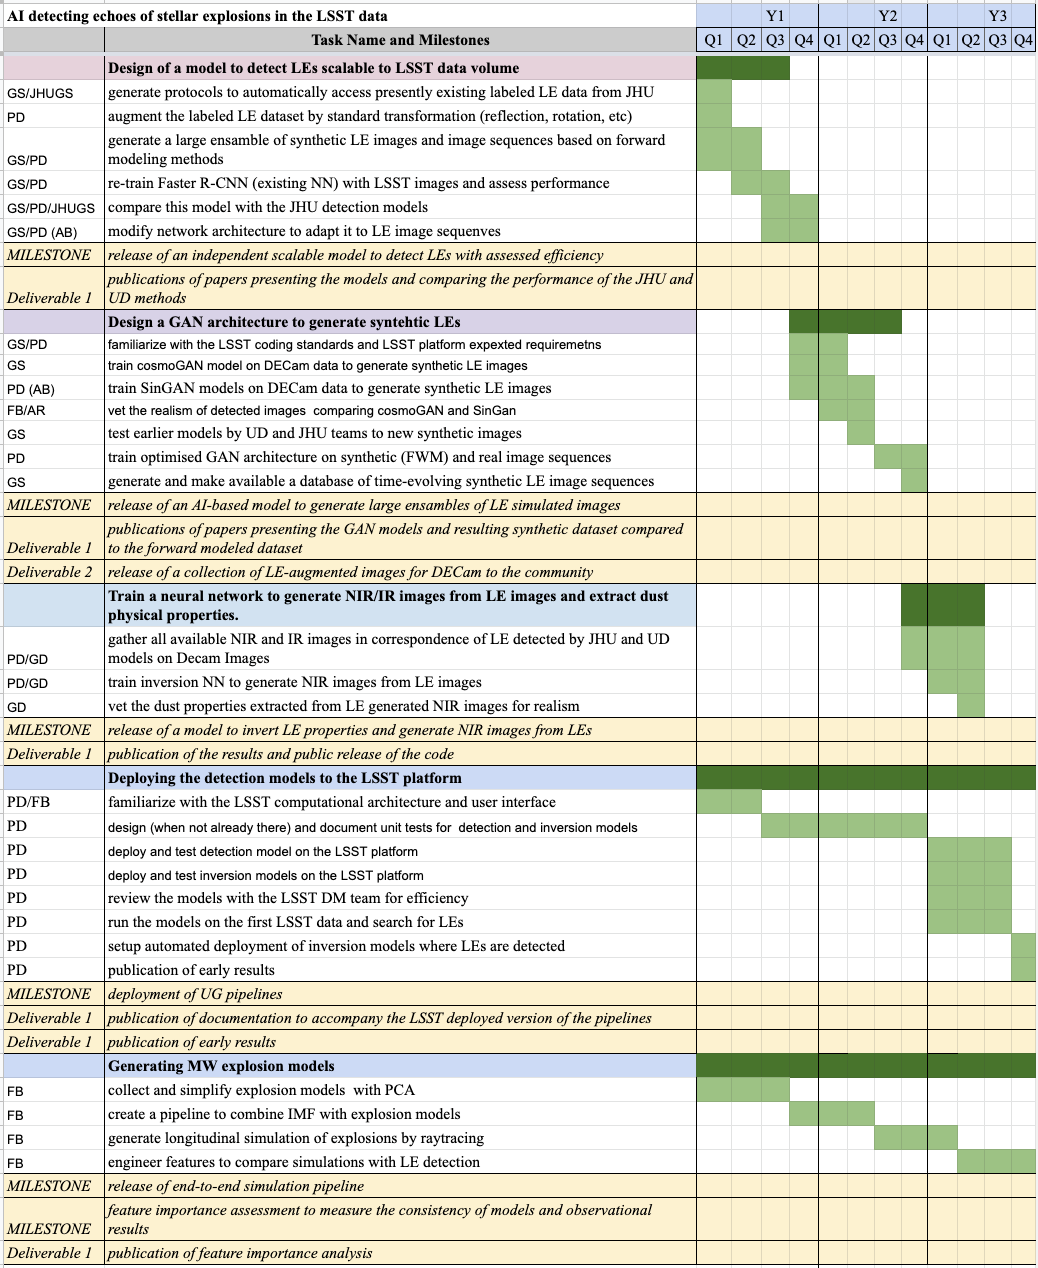
\includegraphics[]{gantt.png}
    \caption{Gantt chart of activities under this proposal}
    \label{fig:gannt}
\end{figure}
 

\subsection{Our team}

{\bf PI Bianco} is a new faculty member at the University of Delaware (UD) Physics and Astronomy Department and Biden School of Public Policy and Administration,  as well as a Resident Faculty member of the new UD Data Science Institute. PI Bianco’s scientific expertise range from data science to data-driven inference in astronomical transients, from nearby Solar System [12] to distant Supernova explosions [13].   She works closely with the team building and scoping the LSST telescope and survey and represents the community working on LSST in various settings (\eg,  recently at the National Academy of Science Space Science Week, invited by the Committee on Astronomy and Astrophysics).  

Among the many transient phenomena in PI Bianco’s research portfolio, she has worked on LEs collaborating with CoI Rest leading the data collection and analysis at the Las Cumbres Observatory Global network, which contributed the majority of the image data analyzed in [3] and focusing on the extraction of lightcurves from LEs that supports the analysis of typing and spectral evolution [19, 20, 24]
and studies that relate diversity in transients to asymmetry as assessed from LEs.  Additionally, she is working on technically similar computer vision issues in the context of urban imaging at the Urban Observatory \changeit[CITE], a multi-city facility lead by Collaborator Dobler where urban environments are studied through imaging and techniques adapted from astronomy (i.e.  photometry, spectroscopy) developing methodology to detect of faint transient diffused feature generated by building HVAC system and other emissions \changeit[CITE].

She will supervise all work and create models of the explosion and eruption history of the Milky way assessing the optimal way to compare them with light echo detections.

{\bf CoI Dr.\ Brockmeier} is a new faculty member at the University of Delaware (UD) in the Departments of Electrical and Computer Engineering and Computer and Information Sciences, and also a Resident Faculty member of the new UD Data Science Institute.  His expertise in signal processing and machine learning include sparse coding for signals, dictionary learning, measures of divergence, signal processing for multimodal data, methods for unsupervised and supervised learning, and neural networks. 

\armin{PLEASE REVIEW}
{\bf CoI Dr. Rest} is a world-renowned expert in LEs, from detection to transient characterization.  He has lead several successfull programs devoted to the study of LEs, including current NSF program 1814993.  He also has lead the acquisition and analysis of light echo data used in this proposal \armin{NOAO PROPOSAL NUMBERS FOR DECAM IMAGES}.  In this project, he will supervise a Graduate student from John Hopkins University in year 1, as well as co-advising the UD Graduate students in developing a detailed work plan and set up the data access, ingestion, and manual labeling to create a standardized dataset of LEs over which the performance of our models will be measured.   


{\bf Collaborator Dr. Peek} developed the forward modeling methodology for LEs and produced several simulations as described in~\autoref{sec:fwm}.  He will make his existing simulations available and coach students in the methodology to create a comprehensive training sample to be fed to our Neural Networks.  

{\bf Collaborator Dr. Dobler} has extensive experience modeling interstellar dust emission, absorption properties, and grain composition as well as the application of machine learning (including neural networks and deep learning algorithms) to ~PB-scale imaging data sets. He will participate in the effort to incorporate dust properties into the analysis and applying machine learning algorithms to simulated data.






\section{Summary: Significance of proposed work}

More text.

\subsection{Intellectual Merit}

More text.
\section{Unfunded Collaborators}

\subsection{CoI Armin Rest, STScI}

Dr. Rest, CoI, and his grad student will contribute to the early phases of the project (y1) by: connecting the results of current NSF funded research on light echoes with the work developed by this team, including sharing data from the KPNO Mosaic II and Mosaic 3, Blanco Mosaic II and DECam, ATLAS systems collected under proposals including NSF grant #128913. Dr. Rest’s JHU graduate student (Roee Partoush) and postdoc (Ryan Ridden-Harper) have started to work on the pipeline and tools to find light echoes in the targeted DECam data, funded by NSF grant #128913. The DECam total data volume is less than just a couple of weeks of the LSST data volume, and therefore the prototype pipeline and tools developed by Dr. Rest’s team need to be further developed for the LSST data. The UD Graduate student working under PI Bianco’s supervision will work closely with Roee Partoush to learn about the DECam tools and adapt what can be used for the LSST pipeline. Rest and his student will help to vet the detection algorithms efficiency and purity with expert knowledge on the detection of light echoes. This is important because, necessarily, the light echoes examples that will be feed to the algorithms  for training and testing can be pure, but not complete (in other words, any real image will contain light echoes that may not have been detected even by accurate visual inspection, as the luminosity of light echoes decreases to 0 without discontinuities).

CoI Rest will provide expertise in later phases of the project at no cost, under his STScI funded responsibility, by helping to create models of explosion and eruption across the Galaxy to be integrated into our pipeline, and designing tests to vet the ability of our models to extract dust properties form light echoes.





\subsection{Collaborator Joshua Peek, STScI}
Peek is an Associate Astronomer and the Data Science Mission Office Project Scientist at the Space Telescope Science Institute.  He developed the forward modeling methodology for LEs and produced several simulations as described in~\autoref{sec:fwm}.  He will make his existing simulations available and coach students in the methodology to create a comprehensive training sample to be fed to our GANs.  

\subsection{Collaborator Gregory Dobler, UDelaware}
Dobler is an Assistant Professor at the Department of Physics and Astronomy, Biden School of Public Policy and Administration, and Data Science Institute at the University of Delaware.   He has extensive experience modeling interstellar dust emission, absorption properties, and grain composition as well as the application of machine learning (including neural networks and deep learning algorithms) to ~PB-scale imaging data sets.   In this project he will participate in the effort to incorporate dust properties into the analysis and applying machine learning algorithms to simulated data, as well as co-supervising the graduate and undergraduate students.

\subsection{Broader Impacts}
The project will involve a University of Delaware graduate student, and it will constitute the core of their thesis.  We will collaborate closely with a Johns Hopkins graduate student in the first year of the project whose thesis is also on light echoes and transient identification in light echoes.  We will involve one undergraduate each year on the project. 

The broader impact of this proposal will focus on machine learning and data science education of undergraduate and graduate students at the University of Delaware (UD) and John Hopkins University. 
This skill are becoming indispensable in an increasingly technological world.  As part of her faculty responsibility toward the Department of Physics and Astronomy (DPA) at the UD, PI Bianco is developing data science and machine learning curriculum for physicists and astronomers (two classes have been developed this year: Data Science for Physical Scientists\footnote{\url{https://github.com/fedhere/dsps}} which is offered at the undergraduate and graduate level, and Machine Learning for Time Series Analysis which will be offered at the graduate level next semester). 
The UD graduate student and the undergraduates involved in this proposal will be encouraged to take these classes, which are project based designed to provide a hands-on learning environment ideal for developing data-driven research skills. 

Projects related to this proposal will offer a research opportunity for undergraduate students that are interested in the new 4+1 Physics and Data Science program at UD. UD launched a Master Degree in Data Science\footnote{https://www.msds.udel.edu/} in 2018 and will expand it to include a 4+1 joint degree with the DPA next year (the 4+1 is under academic review).

Another important opportunity  will be available to all student involved in this proposal (at UD and Hopkins), and to all UD students, through a UD hackathon program that PI Bianco and CoI Brockmeier will start at the UD Data Science Institute.  This program will organize UD-wide hackathons for all UD students at least twice a year.

Hackathon and data dives are prime examples of active learning activities.  We will organize hackathons twice yearly as a weekend long event.  Students will work in self-assembled groups on projects of their choice and produce a deliverable, which they will present at the end of the event in front of judges and a small audience.  Open to all interested undergraduates, the hackathons will have a variety of topics, both proposed by the UD faculty and by the students themselves (LSST-related projects will be made available at each session, including projects related to the research supported by this proposal). This is an ideal venue for building superskills, especially collaborative and communication skills, in our students. LSST has supported hackathons in various environment as a way to jump-start LSST related research and PI Bianco has been involved in the leadership and organization of many of these events (e.g. http://fbb.space/LSSTHackathonCCA/WPgallery.html, https://lsst-tvssc.github.io/TVS-SMWLV2019/).

A typical hackathon event starts with project pitches.  Students are encouraged to present project ideas, but projects are also available and presented by the moderating faculty and postdoc.  Occasionally, external agencies or companies are invited to pitch projects as well.  In that case, they may provide prizes to the winning teams.  A pitch would include a problem statement, the desired deliverable, and the skills required for the project.
Groups self-assemble to work on projects based on interest and required expertise and work continuously, including on the preparation of a 5-10 minutes slides presentation that concludes the event.  During the hackathon, mentors are available to help and advise the students on methodology, and a moderator makes sure the tight timeline is respected, including containing the initial pitches and team assembling time, and assuring that students prepare the slides timely for the presentation. 
Project results are presented by each team.  Feedback is given separately on the presentation, by an assigned "critique", and on the content by the judges, that have priority in asking questions and giving feedback, then time permitting additional questions are asked by the audience.  Projects are ranked based on their success in four main areas: 

- the quality of the presentation

- the quality of the deliverable

- how well the deliverable complies with the request formulated in the pitch 

- the application of adequate and appropriate methodologies.

In these events, the students see the full life-cycle of a data-driven project, from conception to presentation.  This is a rare opportunity for them since in course-based instruction, even in project-based classes, generally the research is guided and extended over time, often resulting in a dispersive, as opposed to immersive, experience. The postdoc hired under this project will serve as a mentor and organizer, together with PI and CoI Bianco and Brockmeier, and as a judge at the final presentation showdown (see Postdoc Mentoring Plan)


\clearpage
\noindent{\Large \bf j Supplementary Material}
\clearpage
\section{Postdoctoral Mentoring Plan - 1 page}

This proposal will support 50\% of the effort of a postdoctoral researcher.  The postdoctoral researcher mentoring plan for this program will be overseen by the PI Dr. Bianco (Assistant Professor at the UD, Physics and Astronomy - DPA) and CoI Dr. Brockmeier (Assistant Professor at the UD, Electrical Engineering).  The different domains of Prof.s Bianco and Brockmeier will provide a complete multi-faceted point of view in reviewing and advising the postdocs on science and job-success related matters. 
The postdoctoral researcher will be recruited with a solicitation issued by PI Bianco on November 2019.  The PIs will create a Postdoctoral Selection Committee including CoI Brockmeier and two senior faculty members within the Department of Physica and Astronomy at UD to review the applications.

To assure that a diverse pull of candidates is reached, PI Bianco has has posted the job announcement on several venues that target diverse scholars (e.g. Diverse Issues in Higher Ed. and Hispanic Outlook).  If a  scholar from an under-represented minority is hired, they will benefit from the commitment of UD and specifically the renewed commitment of the DPA to create an equitable and supportive environment with a new Diversity and Inclusion Committee\footnote{http://bit.ly/UDDPADIcommittee}, created and chaired by PI Bianco at the UD DPA.

The PI and CoI will offer, as part of the mentoring program: 
1) Training in preparation of grant proposals: Being able to effectively and consistently find funding is a compulsory skill required of successful researchers.  The postdoctoral researcher should be coached in and encouraged to submit proposals (e.g. postdoctoral fellowship, HST proposals) and encouraged to serve on at least one review panel to gain a deeper understanding of the review process. 
2) Publications and presentations: The mentors will support (through this grant and her start-up funds) travel support to assure the postdocs can present their work at conferences and publish in high impact journals.  The postdocs should travel to the LSST annual Community Workshop, international LSST meetings (e.g. LSST@Europe, on a bi-annual basis), and topical AI meetings. 
3) Mentoring: The postdoc will have opportunities to interact with and mentor students. They will mentor the graduate and undergraduate students working with PI Bianco and CoI Rest, but the PI will also involve the postdoc in hackathons as mentor, both in LSST meetings and at the UD Data Science Institute, where PI Bianco and CoI Brockmeier are developing a hackathon program of 2 events each year (PI Bianco has experience developing such programs at NYU Center for Urban Science and Progress and elsewhere, see biosketch).  The postdoctoral researcher will be involved in  planning and preparing the hackathons and will serve as mentors during the hackathon sessions and as judges at the hackathon presentations.
4) Career Counselling: A likely outcome for the postdoc is  employment outside of academia: in recent years the number of graduating PhD physics students ranged between 1500 and 2000, while the number of  faculty hires ranges between 200 and 300\footnote{\url{https://www.aip.org/sites/default/files/statistics/physics-trends/fall16-phdsubfield-p1.pdf}}\footnote{\url{https://www.aip.org/statistics/physics-trends/number-faculty-hired-physics-departments}}.  The postdoctoral researcher will data science learning skills that are crucial in the tech job market and will be encouraged to continually discuss their career options with their mentors, peers, and collaborators, so that they can successfully gauge the appropriate skills required for their chosen career path.
Assessment: The personal progress of the postdoctoral researchers will be measured against the expectations laid out in this mentoring plan, i.e.: number of papers and proposals submitted, the number of seminars given, quality of lectures, and  effectiveness of their mentoring (student success).  Every 4 months the postdoctoral research will meet separately with PI Bianco and CoI Brockmeier so that they will be able to raise concerns about mentoring.  Dr. Bianco and Dr. Brockmeier will share a report with the postdoctoral research every 4 months.  


\clearpage


\newpage
\pagenumbering{arabic}
\renewcommand{\thepage} {E--\arabic{page}}

\bibliography{refs}
\bibliographystyle{jponew}

\newpage
\pagenumbering{arabic}
\renewcommand{\thepage} {G--\arabic{page}}
\noindent{\Large \bf BUDGET JUSTIFICATION}

\end{document}
